\chapter{绪论}
\label{chapter:chapter1}
\section{引言}
随着深度学习\cite{lecun2015deep}领域不断取得突破性进展,基于深度学习模型的手机移动应用也如雨后春笋般发展起来。智能手机已经在逐渐改变人们的生活方式,几乎每部手机都集成着若干功能各异的传感器,这些传感器每天都在采集着大量与使用者相关的复杂数据,而深度学习模型无疑是处理这些数据的最佳工具。但是,由于当前嵌入式平台的资源限制(内存、计算能力、电池容量等),基于深度学习模型的应用并没有在手机移动应用市场中成为主流。

虽然深度学习模型对硬件资源的苛刻需求阻碍了它向手机移动平台的“进军”,但是其带来的好处仍然诱惑着人们在物联网设备和移动硬件上采用它。目前,手机上基于深度学习模型的应用(如,图像识别、语音识别)绝大部分都是基于云端服务的,即手机端采集所需的传感数据并通过网络将数据上传到云端服务器,云端服务器在获得数据后,运行深度学习模型推断,最后将所得的推断结果再次通过网络传回至手机端。然而,这种处理方式带来了许多负面影响,主要总结如下:1)它可能会泄露用户的隐私数据,因为它需要将用户的一些敏感数据(如,图像、音频)发送到第三方服务端进行处理;2)它的推断执行时间将会与波动的、不可预测的网络质量(如,网络延迟、吞吐量)紧密挂钩。更糟糕的是,当网络条件很差甚至不可联网时,这种推断操作就不能正常进行;3)由于无线通信能量开销的存在,对于那些需长时期运行的应用(如,增强现实、认知助理等),使用云端执行推断任务也是不切实际的;4)因为移动网络是按流量收费的,所以用户就不会使用那些需发送大量待处理数据(如视频流)至云端的应用,这便限制了深度学习模型在移动端的应用场景。

考虑到上述云端执行的负面影响,用户可能更希望那些基于深度学习模型的应用在手机本地就可以完成推断任务。另一方面,我们需要意识到高能效移动处理器的计算性能一直处于不间断地发展中。例如,与4年前的iPhone 5S相比,2017年苹果发布的iPhone 8在CPU单核处理性能上拥有着232\%的增长,而在多核处理性能上更是提高了373\%。许多研究学者认为,在不久的将来,即使没有远程计算的辅助,手机移动端也可以胜任许多基于深度学习模型的计算任务。通过手工改造并简化深度学习模型(如卷积神经网络\cite{krizhevsky2012imagenet}),在移动端本地设备上直接运行一些深度学习模型已经被证明是可行的,但是这样做不但需要大量的设计技巧,而且对于现存的大多数深度学习模型来说都是行不通的。更为重要的,正是因为深度学习模型的复杂性才使得推断准确度和鲁棒性取得了革命性的飞跃,并且这才是智能移动应用所迫切需要的,所以手工简化模型的方式并非是我们的初衷。

与桌面、服务器端相比,手机移动端的不足不仅表现在较弱的处理能力上,还凸显在较小的内存容量上(如,华为Mate 9 Pro的内存容量仅为4GB)。然而,因为深度学习模型具有结构异常复杂的特点,所以绝大部分模型都拥有着成百万上千万甚至上亿的参数(如,VGG16\cite{simonyan2014very}模型拥有1.8亿个参数)。这导致了许多深度模型并不能在手机移动端运行。而且,即使一些模型可以运行,其也会造成大量的内存占用和能耗开销。

综上所述,采用深度学习模型处理移动传感数据并在移动端进行离线推断是未来手机移动应用发展的一种趋势。为了将这一趋势转变为现实,当前研究人员必须要对移动端深度学习模型的本地推断过程进行各种能效优化。目前,研究工作需要解决的主要问题总结如下:

\begin{enumerate}
\item  如何利用当前移动设备处理器的特点及其未来的发展趋势,使得深度学习模型可以高能效地于移动端进行离线推断。
\item 受限于当前手机内存容量较小的不足,如何使得结构复杂的深度学习模型也可以正常地在移动端运行。
\item 在保证性能的条件下,如何根据应用场景的特点和系统层提供的信息,进一步降低上层基于深度学习模型应用的运行时功耗和能耗。
\end{enumerate}

\section{深度学习模型于移动端能效优化的研究现状}
\subsection{早期的探索与尝试}
Lane等人\cite{lane2015can}设计了一个基于移动设备CPU和DSP的低功耗深度神经网络(DNNs)\cite{deng2013new}原型推断系统。他们利用该推断系统研究了一些典型的移动感知任务(如行为感知),并将该推断系统与更加通用的传统辨识技术(如SVM、GMM和决策树等)相比较。他们的研究表明推断系统中所使用的深度神经网络并不会给现代的移动硬件带来过度的负载压力,而且即使是一个简单的DNN模型(如减少71倍的输入特征数),与传统的通用学习技巧相比,也可以改善推断精度。Lane等人\cite{lane2015early}还研究了一些深度学习模型(DNNs和CNNs)在按比例缩小后,在资源受限的嵌入式设备上执行推断阶段的运行时行为和资源特征。Yanai等人\cite{yanai2016efficient}探究了适合在移动端实现的CNN结构,并提出了多可扩放的Network-In-Network(NIN)\cite{lin2013network},即用户可以调整识别时间和识别精度的折中比。他们的研究发现BLAS库适合加速IOS系统上卷积层的计算,而NEON SIMD\cite{mitra2013use}更适合在Android系统上加速卷积层的计算。
\subsection{基于模型压缩的优化}
Denton等人\cite{denton2014exploiting}通过使用线性压缩技巧去除了CNN模型中的冗余参数,有效地加速了大型已训练CNN模型的推断执行速度,而为此只需要付出很小的推断精度损失。类似地,Jaderberg等人\cite{jaderberg2014speeding}利用不同特征通道和卷积核间存在的冗余特征对卷积核进行了低秩近似分解。Lebedev等人\cite{lebedev2014speeding}使用非线性最小平方法计算一个四维卷积核的低秩CP-分解,即使用一些秩为1的张量之和表示该四维卷积核。Wu等人\cite{wu2016quantized}提出了一个量化的卷积模型,可以在加速计算的同时降低模型的存储和内存开销。Wang等人\cite{wang2016accelerating}使用一个基于低秩的、分组稀疏向量分解的方法加速CNN模型的推断阶段。该方法的核心思想是将卷积核分解为一些小数量的多线性低秩张量之和,并用这些近似张量代替原始的卷积核执行标准回传过程以微调模型。
\subsection{基于异构计算的优化}
为了验证使用移动端GPU执行卷积模型推断的加速效果,Lokhmotov等人\cite{lokhmotov2016optimizing}基于三星 Chrome-book 2平台分析了AlexNet\cite{krizhevsky2012imagenet}卷积模型的前向推断在移动端的执行性能。根据实验结果,他们发现带有OpenBLAS\cite{xianyi2012openblas}支持的Caffe\cite{jia2014caffe}要比带有ViennaCL\cite{rupp2010viennacl}支持的Caffe快大约4倍,比带有clBLAS\cite{nugteren2017clblast}支持的Caffe快大约10倍。他们认为这可能是因为当前移动端的GPU性能较差,并且支持OpenCL\cite{stone2010opencl}的现有并行库没有针对移动端进行优化。DeepX是Lane等人\cite{lane2016deepx}为在移动平台上运行深度学习模型设计的一个软件加速器。DeepX利用一个基于网络计算(远程处理器)和本地异构处理器的混合体(包含CPUs,GPUs,LPUs等)来降低资源的开销。DeepX通过两个推断时资源控制算法来提升性能,即运行时层压缩和深度结构分解。然而,DeepX主要缺点有两点:(1)运行时层压缩不仅没有减少运行时的内存开销,还加重了处理器的计算量;(2)运行时所使用的一些决策参数来源于离线计算好的值,不能适应运行环境的变化。Huynh等人\cite{huynh2016deepsense}设计了一个基于手机GPU的深度神经网络框架DeepSense。DeepSense是基于OpenCL的,故而可以在GPU上执行CNN模型推断。然而,其计算密集型的操作(如,卷积运算)主要运行在GPU上,没有充分利用CPU的多核处理能力。与此同时,DeepSense不支持模型压缩,这使得一些大而复杂的模型不能正常运行。文献\cite{latifi2016cnndroid}呈现了一个基于GPU加速的库(CNNdroid),其主要使用Android官方提供的高性能计算框架RenderScript\cite{guihot2012renderscript}来加速已训练CNN模型的推断过程。然而,其同样没有对一些较大的模型做压缩处理。
\subsection{其他优化方法}
除了上述三类研究外,还有一些其他的相关研究。文献\cite{lane2015deepear,chen2014small,variani2014deep}通过按比例缩小深度模型的方法,将深度学习模型缩小后运行在手机或DSP上。使用低功耗处理器也被证明对于连续传感类型的应用特别有效,该类系统诸如Speakersense\cite{lu2011speakersense}、Dsp.ear\cite{georgiev2014dsp}等,它们在应用级进行优化以均衡主处理器和协处理器间的负载。Antoniou等人\cite{antoniou2016general}将深度卷积模型应用在智能监控系统中,分别于PC和移动设备上实现了一款可以自动检测、智能识别的在线监控系统。最后,开发深度学习领域的专用硬件是另外一个当前较为热门的研究方向,许多研究人员对此做出了贡献,如Diannao\cite{chen2014diannao}以及FPGA神经网络加速器\cite{zhang2015optimizing,wang2017dlau,yu2015deep,wang2016solar}等。

可以看出深度学习模型于手机移动端的应用是近两年刚刚兴起并快速升温的研究方向。然而,大量研究学者的关注点都是放在如何提高深度学习模型于移动端的运行速度,而本课题的研究重点更多的是能效兼顾,并且会着重考虑能耗问题。

\section{论文的主要研究工作}
本文主要针对当前已被工业界广泛应用的深度卷积神经网络模型(CNNs)在Android平台上的推断执行进行能效优化研究,且主要工作包含以下方面:
\begin{enumerate}
\item 分析卷积神经网络进行前向推断时所需的基本算子,并通过OpenCL异构编程框架在手机GPU上实现计算密集型的算子。离线解析经Caffe、YOLO\cite{redmon2016you}和Tensorflow\cite{abadi2016tensorflow}等深度学习框架训练得到的卷积神经网络模型权重并将这些权重保存成统一的格式,以便在移动端重构不同框架训练出来的CNN模型。
\item 在保证推断精度损失极少的条件下,使用“剪枝-重训”算法对预训练好的CNN模型权重参数进行压缩,这样不仅可以降低网络模型的存储占用,还减少了模型内存加载时间和重构过程中的访存能耗。针对剪枝得到的稀疏矩阵,使用稀疏矩阵向量乘代替内积操作,进一步加快卷积神经网络的前向推断速度。
\item 为了充分利用当前以及未来移动设备SoC所提供的异构计算特征,本文提出了一种简单有效的方法,使得基于CNN模型的应用在运行时可以根据其所处运行环境中CPU、GPU等异构设备处理器的推断能效差异,自适应地寻找一个高能效的本地异构处理器组合并行执行CNN前向推断。
\item 针对需长时期运行的CNN模型应用(Life-logging Apps),本文通过离线分析其运行时负载特征进一步探索在系统层使用动态电压频率调节技术(DVFS)\cite{le2010dynamic}提高该类应用性能或能效的策略。
\end{enumerate}

通过上述第1、2、3点优化策略,本课题设计与实现了一套可高能效运行在Android平台的CNN推断时库,并最终将其运用在一个生活日志型应用(如智能监控系统)中以验证第4点优化策略的有效性。图\ref{figure:figurework}描述了本课题研究工作的技术路线。

\begin{figure}[htbp]
    \begin{center}
    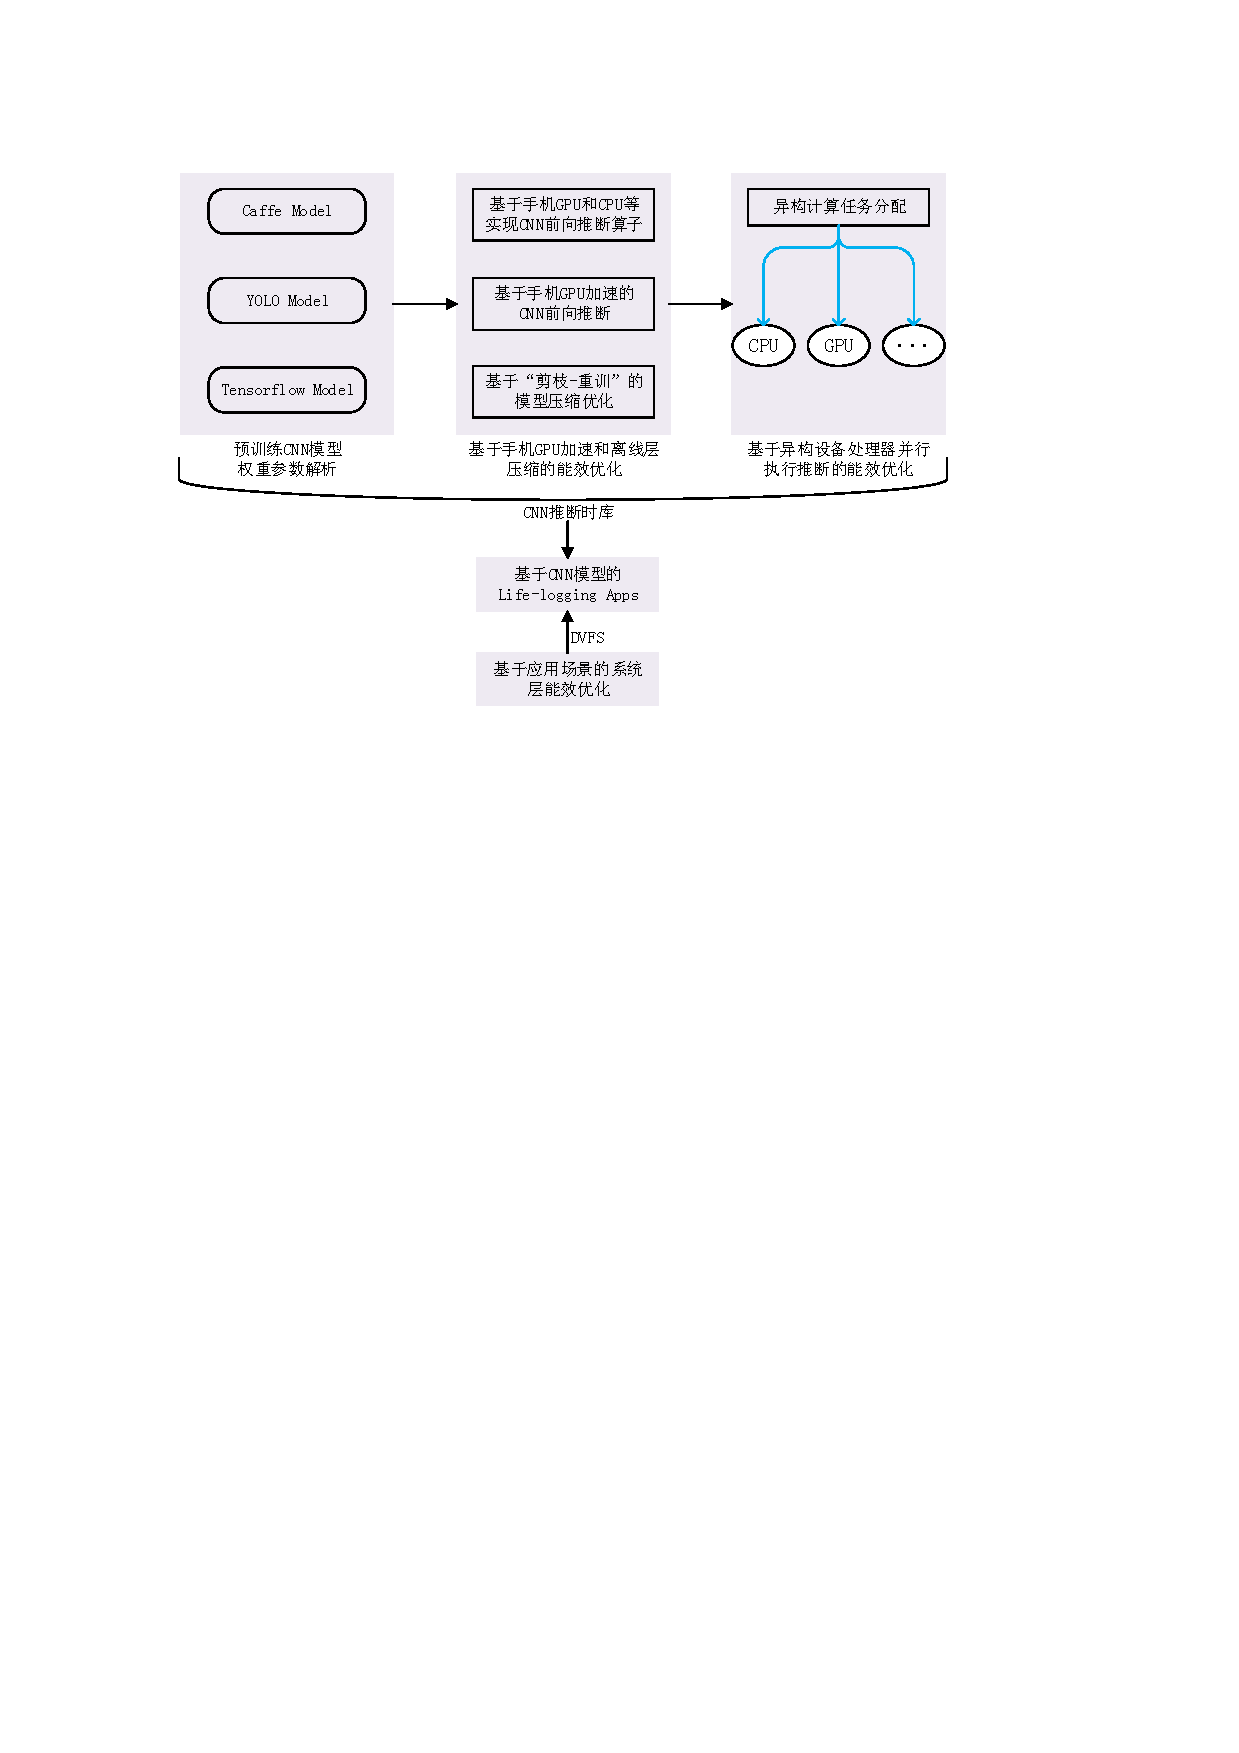
\includegraphics[width=1.0\textwidth]{figures/work.pdf}
    \end{center}
    \caption{研究工作的技术路线}\label{figure:figurework}
\end{figure}

\section{论文的组织结构}

本文的章节安排如下:

第\ref{chapter:chapter1}章主要讲述了深度学习模型在手机移动平台上的应用现状,并分析了阻碍基于深度学习模型移动应用发展的原因以及使用手机本地离线推断的必要性。接着,通过详细介绍深度学习模型于移动端进行能效优化的研究现状,引出本文的研究内容与目标。

第\ref{chapter:chapter2}章首先介绍了卷积神经网络的相关概念和组成结构,并对反向传播算法中所使用的梯度下降法和反向传播过程进行了阐述。然后,介绍了OpenCL异构编程框架的基本概念与开发优点,并给出了基于该框架的异构程序设计流程。最后,描述了本文中所采用的能效度量标准并详细介绍了本研究中所使用的实验平台。

第\ref{chapter:chapter3}章首先对卷积神经网络前向推断过程中所使用的基本算子进行了分解,并详细描述了这些算子的作用与原理。然后,分别给出了这些基本算子在手机GPU和CPU上的实现方法。接着,描述了基于“剪枝-重训”的权重压缩方法,并使用该方法对卷积神经网络中占存储量主要部分的全连接层权重进行了压缩。对于压缩后的网络,进一步使用稀疏矩阵向量乘(SpMV)代替密集矩阵的内积运算,并给出了SpMV在移动端的实现。最后,基于Caffe、YOLO和Tensorflow等深度学习框架所训练的CNN模型权重,本文在移动端重构了LeNet-5\cite{lecun1998gradient}模型和AlexNet模型,并比较分析了基于手机CPU、手机GPU和基于SpMV实现之间的能效差异。

第\ref{chapter:chapter4}章首先探讨了当前移动端SoC的发展趋势。接着,全面分析了在手机GPU和CPU上分别执行CNN前向推断时的能效,进而阐述了利用所有可获得的手机本地处理器去执行CNN前向推断并非是一种高能效的方式。本文提出一种简单有效的方法,其可以自适应地评估特定移动平台上所有可获得的本地处理器的能效,并进一步通过计算得到一个高能效的设备处理器组合用以并行执行CNN的前向推断过程\cite{wang2017rethinking}。最后,本文使用一种基于不同处理器计算性能的方法为所选组合中每一个设备处理器分配计算任务。

第\ref{chapter:chapter5}章首先介绍了动态电压频率调节技术(DVFS)的相关概念,并基于第\ref{chapter:chapter2}、\ref{chapter:chapter3}、\ref{chapter:chapter4}章节设计的CNN推断时库开发了一款生活日志型Android应用——智能监控系统。针对该应用,本文从系统层详细分析了其负载特征,并探索了利用DVFS技术进一步提高该类应用性能或能效的策略。

第\ref{chapter:chapter6}章对全文进行了总结,并对论文中尚未解决的问题提供研究线索,以期在未来的工作中加以解决并完善。

\cleardoublepage 